\documentclass[
	%a4paper, % Use A4 paper size
	letterpaper, % Use US letter paper size
]{jdf}

\addbibresource{references.bib}

\author{Yicun Deng}
\email{ydeng335@gatech.edu}
\title{Project6: \\Seeing the Future and Cheat}

\begin{document}
%\lsstyle

\maketitle

\begin{abstract}
	This project forms the foundation for future work by developing five technical indicators and a Theoretically Optimal Strategy (TOS) that maximizes portfolio returns. We delve into the methodology, statistical performance, and visual representation of these components, contrasting the TOS against a benchmark. These outcomes pave the way for future application of machine learning in trading strategies, serving as a pivotal resource for understanding financial market analytics.
\end{abstract}
	

\section{Background}
This project is developed and tested in an Windows Subsystem of Linux environment with ML4T conda environment. Packages: Numpy, Pandas, Datetime, Matplotlib

\subsection{Introduction}

This research analyzes trading strategies with a dual focus: evaluating five technical indicators (Bollinger Bands Percentage (BBP), Percentage Price Oscillator (PPO), Moving Average Convergence Divergence (MACD), Stochastic Oscillator (SO), and the Golden Cross (GC)), and showcasing a Python-based trading algorithm. The indicators, each providing unique insights on market trends, are studied for their impact on trading outcomes. Our algorithm, utilizing historical stock prices, aims to optimize trading strategy by predicting buy and sell signals. The study serves financial analysts, quantitative traders, and anyone interested in the practical application of algorithmic trading strategies.

\section{Experiment}
Both the indicators section and optimal strategy section uses data of 'JPM' between 2008-1-1 and 2009-12-31 for following instruction and aligning for analysis purpose.

\subsection{Indicator Analysis}

In this section, we delve into our choice of five technical indicators, elucidating their mathematical computation, their potential utility in signaling buy or sell decisions, and the methodology used to standardize them for our analysis. Each indicator is dissected, and their characteristics over time for a specific stock are portrayed visually. We also shed light on our Python implementation used for the computation of these indicators.

\begin{jdftable}
\captionof{table}{Performance of Trading Indicators}\label{table:Indicators}
\small % Reduce font size
\begin{tabular}{@{} L{0.35\linewidth} S}
		\textbf{Indicator} & \textbf{Correlation with Optimal BUY/SELL} \\
		\toprule[0.5pt]
		Bollinger Band Percent (BBP) & 0.272897 \\
		\midrule
		Percentage Price Oscillator (PPO) & 0.047342 \\
		\midrule
		Moving Average Convergence Divergence (MACD) & 0.128009 \\
		\midrule
		Stochastic Oscillator (SO) & 0.304577 \\
		\midrule
		Golden Cross (GC) & 0.023337 \\
\end{tabular}
\end{jdftable}

We assessed the efficacy of our indicators by correlating them with optimal buy/sell signals, as displayed in Table \ref{table:Indicators}. This integrative strategy merges the indicators' benefits with our optimal approach, offering a comprehensive view of the market and reinforcing our trading strategy.

\subsubsection{Fundamental Math for Indicators}

The Simple Moving Average (SMA) averages the price over a defined number of periods, typically closing prices. Formally:
{\small
\[
SMA = \frac{\sum_{i=1}^{n}Price_{i}}{n}
\]
}
where $Price_{i}$ is the price at period $i$, and $n$ is the number of periods.

The Exponential Moving Average (EMA) gives more weight to recent prices, reducing lag. It's calculated as:
{\small
\[
EMA_{t} = (1-\alpha) \cdot EMA_{t-1} + \alpha \cdot Price_{t}
\]
}
where $\alpha = \frac{2}{N+1}$ is the smoothing factor and $N$ is the length of the window.

Finally, we standardize our indicators to be roughly normally distributed by subtracting the mean and dividing by the standard deviation. This is formulated as:
{\small
\[
Z = \frac{X - \mu}{\sigma}
\]
}
where $Z$ is the standardized score, $X$ is the raw score, $\mu$ is the mean, and $\sigma$ is the standard deviation.

	
\subsubsection{Bollinger Bands Percentage (BBP)}

Bollinger Bands Percentage (BBP) was chosen for its ability to measure price volatility. It calculates the relative position of a stock's price in relation to the Bollinger Bands. The mathematical representation of BBP is as follows:

\[
BBP = \frac{Price - Lower\ Band}{Upper\ Band - Lower\ Band}
\]

where, 
\[
Upper\ Band = Rolling\ Mean + (2 * Rolling\ Standard\ Deviation)
\]
\[
Lower\ Band = Rolling\ Mean - (2 * Rolling\ Standard\ Deviation)
\]


The Bollinger Band Percent (BBP) is a technical indicator offering insights into potential buying or selling opportunities. Its values range from 0 to 1, where numbers closer to 1 suggest a selling opportunity and those near 0 signal a buying possibility. Following standardization, BBP values revolve around 0. Positive values hint at selling opportunities and negative ones at buying.

\begin{jdffigure}
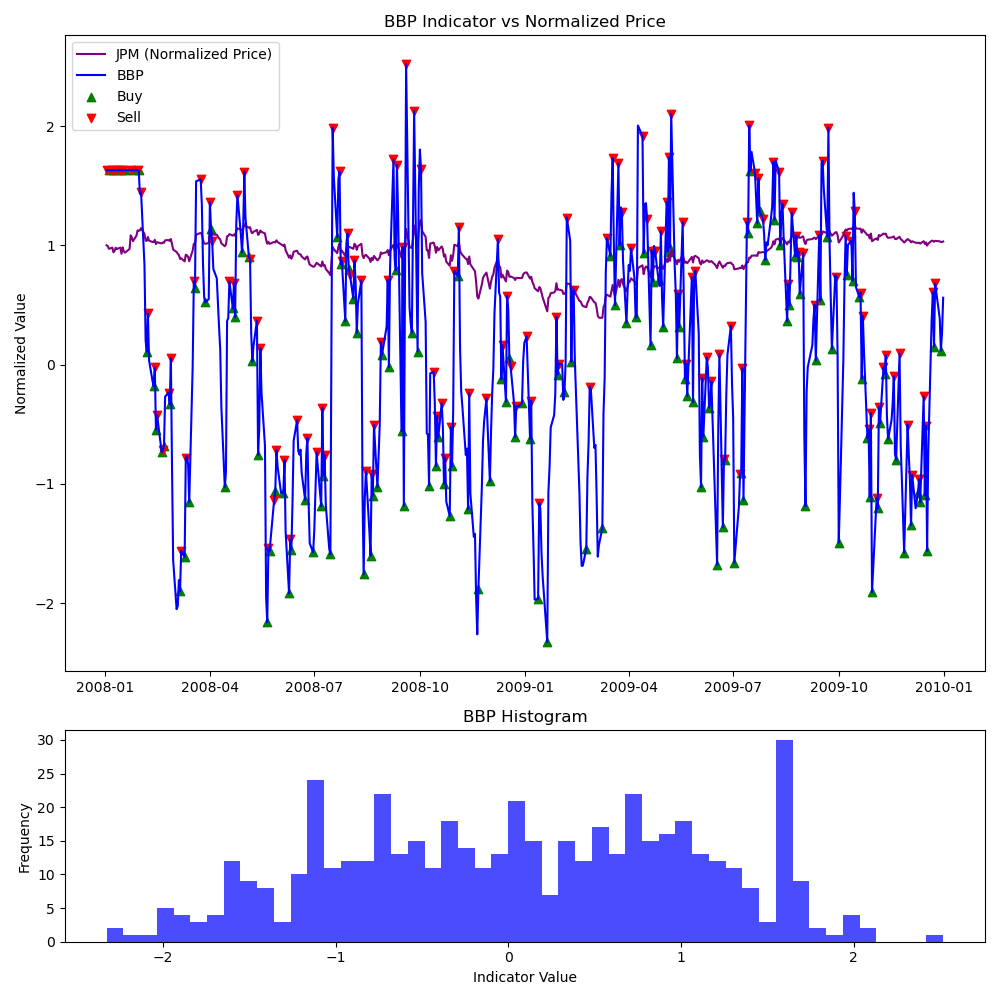
\includegraphics[height=6cm]{Figures/BBP_hist_and_price.png}%
\captionof{figure}{Bollinger Band Percent (BBP) Indicator Over Time. This figure visualizes the calculated BBP values for a specific stock over the observed period. It illustrates periods of overbuying and overselling, which are indicative of potential trading opportunities.}\label{fig:BBP}%
\end{jdffigure}
	

As shown in Figure \ref{fig:BBP}, BBP values for a specific stock over the period under observation reflect periods of overbuying and overselling, thus providing potential trading cues. In our study, BBP values nearer to 2.0 signal selling, while those closer to -2.0 suggest buying. However, with a correlation of 0.27 (refer to Table \ref{table:Indicators}), the indicator has only a modest predictive power and isn't potent enough to serve as a standalone trading guide. Additionally, despite a slight surge around 1.75 in the BBP distribution, this isn't a strong nor interpretable signal for trading. Therefore, it underscores the need for an ensemble of indicators for a more robust trading strategy.



\subsubsection{Percentage Price Oscillator (PPO)}

The Percentage Price Oscillator (PPO) is another key indicator we opted for due to its proficiency in revealing the relationship between two moving averages. The PPO is essentially a percentage comparison of two Exponential Moving Averages (EMA) - one short-term and one long-term. This comparison is specifically valuable as it can help identify potential price momentum shifts and trend reversals.

Mathematically, it is calculated using the formula:
\[
PPO = \frac{EMA_{short} - EMA_{long}}{EMA_{long}} * 100
\]

where $EMA_{short}$ is the short-term Exponential Moving Average and $EMA_{long}$ is the long-term Exponential Moving Average. By standardizing the difference between the two EMAs to a percentage, the PPO allows for comparability across different securities and timeframes.

In trading contexts, a positive PPO value, where the short-term EMA is greater than the long-term EMA, could indicate a buying opportunity as it signifies upward momentum. Conversely, a negative value, where the short-term EMA is lesser than the long-term EMA, could signal a selling opportunity due to downward momentum.

An important aspect of the PPO is the zero line. When the PPO crosses the zero line from below to above, it indicates a bullish (buy) signal, while crossing from above to below signals a bearish (sell) stance. However, as with any single indicator, these signals should not be used in isolation and should be validated with other indicators and market analysis.

\begin{jdffigure}
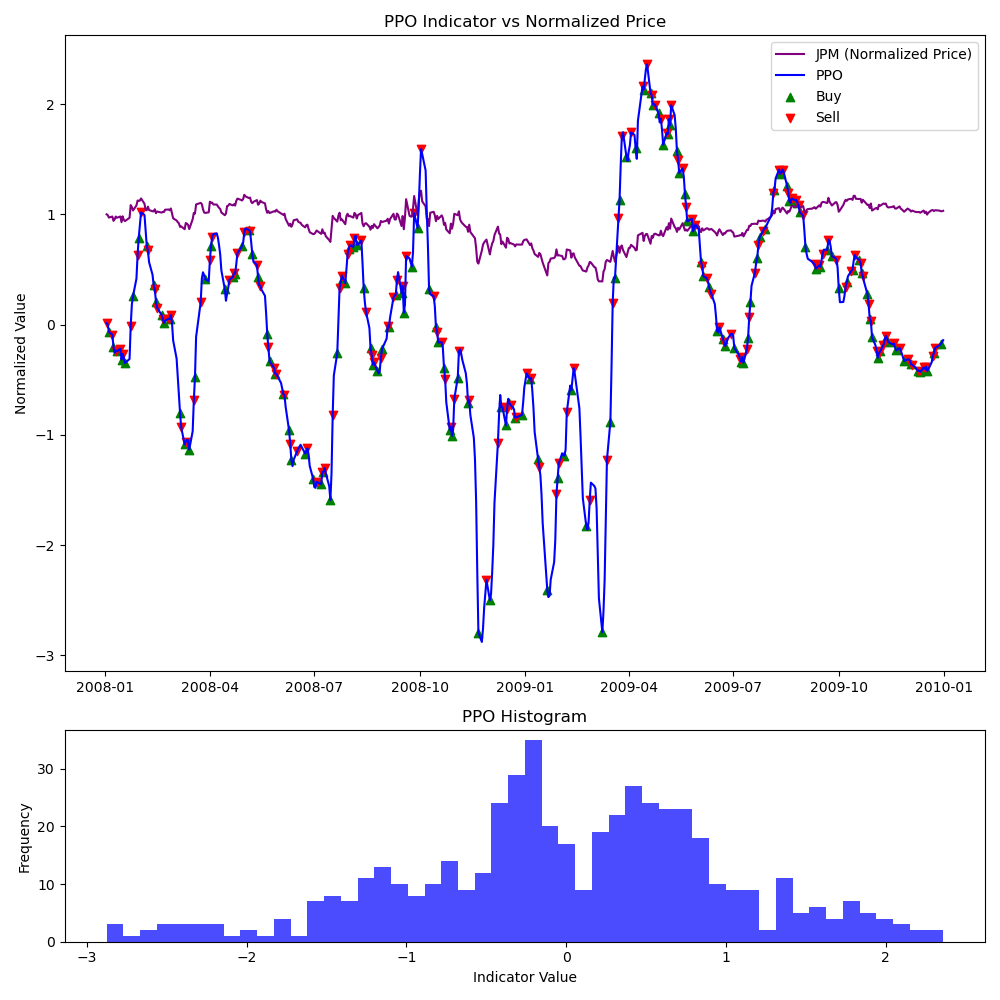
\includegraphics[height=6cm]{Figures/PPO_hist_and_price.png} \\
\captionof{figure}{Percentage Price Oscillator (PPO) values for the stock over time. The figure highlights potential buying (positive PPO) and selling (negative PPO) signals, aligned with the zero-centered distribution after standardization.}\label{fig:PPO}%
\end{jdffigure}

The Percentage Price Oscillator (PPO) is a momentum-based indicator that provides a perspective on the rate of change in a security's price. Despite its seemingly low correlation of 0.047 with optimal buy/sell signals, as depicted in Table \ref{table:Indicators}, it serves as a useful tool when used in conjunction with other indicators.

PPO's strength lies in its ability to standardize momentum, allowing comparative analysis across diverse securities and timeframes. Nevertheless, as a standalone indicator, its effectiveness in triggering trade decisions appears limited, likely due to the potential for false signals and its inability to account for unforeseen market events. Therefore, using the PPO as part of a multifaceted trading strategy, rather than a singular predictive tool, is recommended.
	
\subsubsection{Moving Average Convergence Divergence (MACD)}

MACD is a trend-following momentum indicator. The mathematical computation is as follows:

\[
MACD = EMA_{short} - EMA_{long}
\]
\[
Signal = EMA_{MACD}
\]

\begin{jdffigure}
	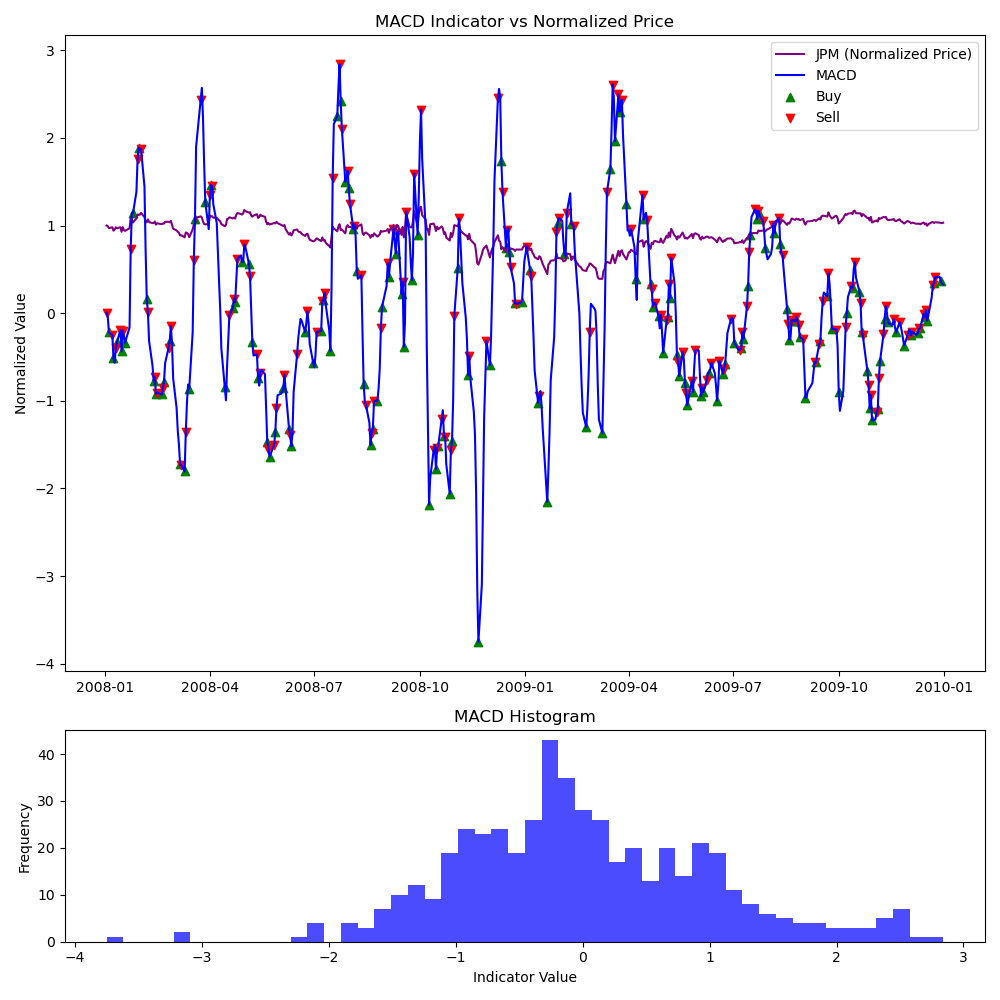
\includegraphics[height=6cm]{Figures/MACD_hist_and_price.png} \\
	\captionof{figure}{Moving Average Convergence Divergence (MACD) histogram values for the stock over time. The figure highlights potential buying (positive MACD) and selling (negative MACD) signals, aligned with the zero-centered distribution after standardization.}\label{fig:MACD}%
\end{jdffigure}
	
Under this analysis, a buy signal may occur when the MACD line crosses above its signal line, indicating bullish momentum. Conversely, a sell signal might be triggered when the MACD line falls below its signal line, signaling bearish momentum. However, the relatively weak correlation of 0.128 (table \ref{table:Indicators}) between these MACD signals and actual trading points suggests that this specific 9-day MACD parameter may not consistently provide accurate signals for this stock during the analyzed period Figure \ref{fig:MACD}. Multiple factors, such as the market conditions and the selected parameters, could contribute to this discrepancy. Therefore, for a more accurate prediction of buy or sell points, it's recommended to use the MACD in conjunction with other trading indicators. In addition, the standardize process might remove some of the information from the original data, which could also contribute to the low correlation.

\subsubsection{Stochastic Oscillator (SO)}

The Stochastic Oscillator (SO) is a momentum indicator comparing a particular closing price of a security to a range of its prices over a certain period of time. It is calculated as:

\[
SO = \frac{Price - Low_{n}}{High_{n} - Low_{n}}
\]

\begin{jdffigure}
	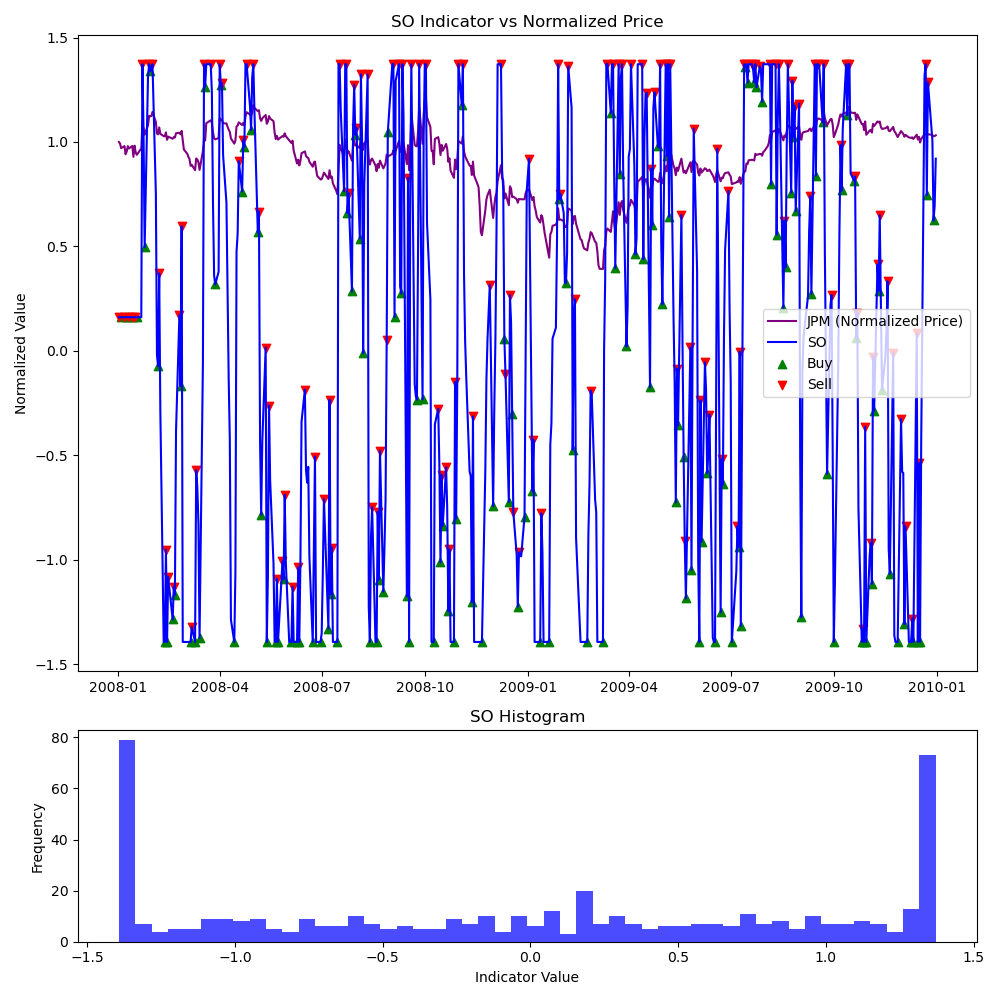
\includegraphics[height=6cm]{Figures/SO_hist_and_price.png} \\
	\captionof{figure}{Stochastic Oscillator (SO) values for the stock over time. The figure highlights potential buying (oversold condition - below 20) and selling (overbought condition - above 80) signals, aligned with the 0 to 100 value range of the oscillator.}\label{fig:SO}%
	\end{jdffigure}

	
where $High_{n}$ and $Low_{n}$ are the highest and lowest prices over a given window. A SO value above 0.8 may suggest the stock is overbought, hence a potential sell signal, while a value below 0.2 may indicate the stock is oversold, implying a potential buy signal. The SO values for a specific stock over the period under observation are depicted in Figure \ref{fig:SO} where it has a tight relationship to our optimal buy or sell. While the standardized SO has a high volatility, its distribution is the opposite of normal which makes it a perfect indicator for trading. The correlation of 0.304577 (table \ref{table:Indicators}) between these SO signals and actual trading points suggests that this specific 14-day SO parameter may consistently provide accurate signals for this stock during the analyzed period. Therefore, the SO indicator is a useful tool for traders to identify potential buy or sell points.

\subsubsection{Simple Moving Average (SMA)}

The Simple Moving Average (SMA), fundamental to the Golden Cross (GC) indicator, is used in technical analysis to filter out short-term price fluctuations, offering a clearer view of price trends. The SMA calculates the average of a selected range of prices over a specific period.


\subsubsection{Golden Cross (GC)}

The Golden Cross (GC) is a candlestick pattern that is a bullish signal in which a short-term moving average crosses above a long-term moving average. It is represented as:

\[
GC = \frac{SMA_{short} - SMA_{long}}{StandardDeviation}
\]

\begin{jdffigure}
	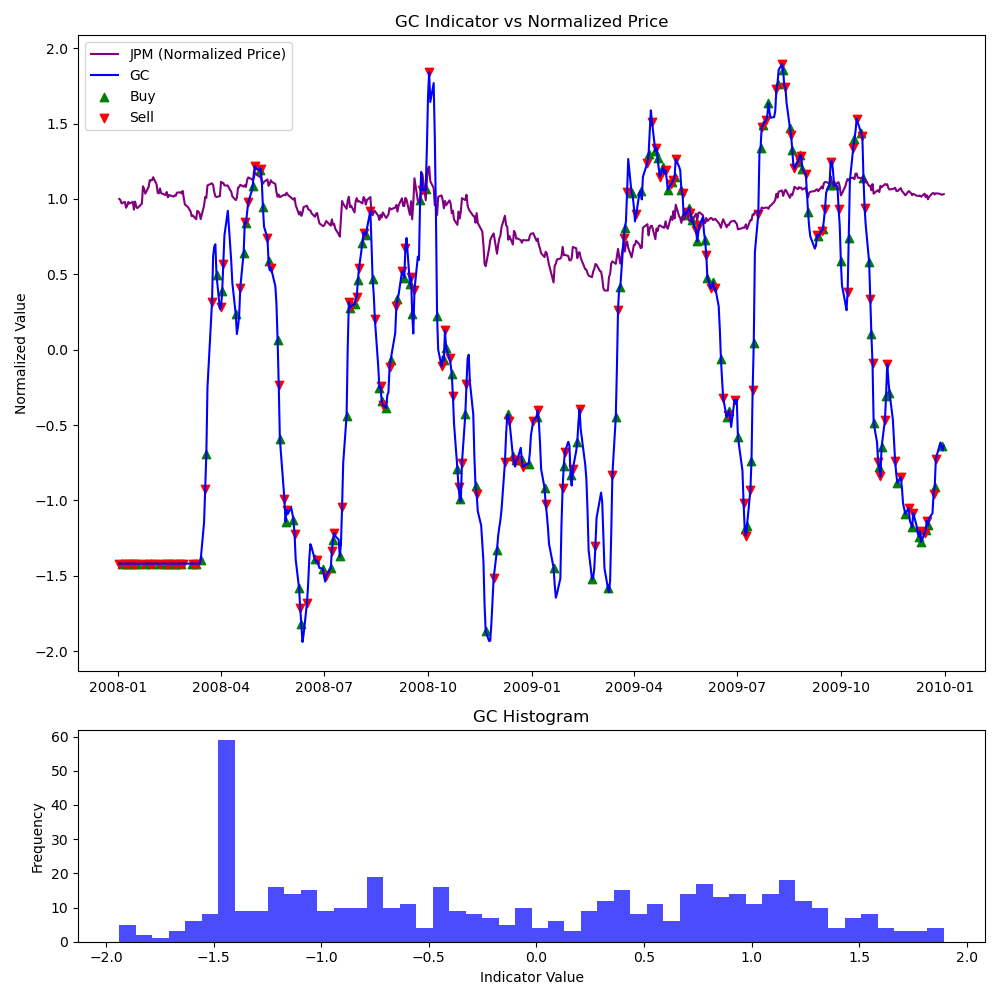
\includegraphics[height=6cm]{Figures/GC_hist_and_price.png} \\
	\captionof{figure}{Golden Cross (GC) values for the stock over time. The figure highlights potential buying (when the short-term SMA crosses above the long-term SMA) and selling (when the short-term SMA crosses below the long-term SMA) signals.}\label{fig:GC}%
	\end{jdffigure}


Figure \ref{fig:GC} depicts the Golden Cross (GC), calculated using a short-term Simple Moving Average ($SMA_{short}$ with a window of 5 days) and a long-term Simple Moving Average ($SMA_{long}$ with a window of 50 days). A positive GC, when $SMA_{short}$ surpasses $SMA_{long}$, might suggest a buying signal, whereas a negative GC, indicating $SMA_{short}$ falling below $SMA_{long}$, might imply a selling signal.

However, the correlation between GC and optimal buy/sell signals in our model is very low (0.023), as shown in Table \ref{table:Indicators}. This suggests the standalone predictive power of GC may be limited, likely due to the delay inherent in SMA-based indicators that can miss rapid market changes.

Despite this, the GC remains useful in detecting long-term trends and may serve to verify signals from other, more reactive indicators. This reinforces the concept of using a diverse set of indicators for a more comprehensive and robust trading strategy.

\subsection{Optimal Strategy}
In this section, we delve into the methodology, statistical performance, and visual representation of our Theoretically Optimal Strategy (TOS). The TOS is a dynamic strategy designed to maximize portfolio returns. In contrast to a benchmark buy-and-hold strategy, the TOS exploits daily fluctuations in price to generate buy and sell signals. 

\subsubsection{Fundamental Logic for TOS}
The key to the TOS is predicting the direction of future price movements. If we expect the price to increase the next day, we aim to maintain a long position. If we are currently short, we first buy to cover our short position and then buy additional shares as long as our available cash permits. Conversely, if we expect the price to decrease the next day, we aim to have a short position. If we are currently long, we sell our position and then continue to sell short as long as our cash reserves allow.

\subsubsection{Result and Analysis}

The results are presented in the table below:

\begin{jdftable}
\small %
\captionof{table}{Performance Metrics of the Benchmark and the Optimal Strategy}\label{table:performance_metrics}
\begin{tabular}{@{} L{0.35\linewidth} S S}
\textbf{Statistic} & \textbf{Benchmark} & \textbf{Optimal Strategy} \\
\toprule[0.5pt]
Start Value & 100000.00 & 100000.00 \\
\midrule
Final Value & 101230.00 & 678440.00 \\
\midrule
Sharpe Ratio & 0.156918 & 13.365085 \\
\midrule
Cumulative Return & 0.012300 & 5.784400 \\
\midrule
Std Dev of Daily Returns & 0.017004 & 0.004551 \\
\midrule
Average Daily Return & 0.000168 & 0.003831 \\
\midrule
Ending Value Ratio of Portfolio & 1.012300 & 6.784400 \\
\bottomrule[0.5pt]
\end{tabular}
\end{jdftable}


\begin{jdffigure}
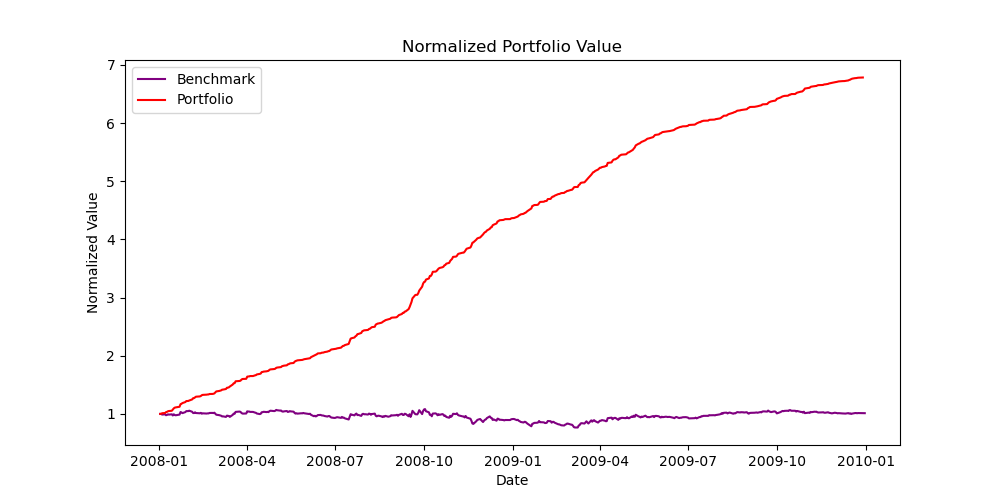
\includegraphics[height=6cm]{Figures/portfolio_value.png}%
\captionof{figure}{Normalized Portfolio Value.}\label{fig:portfolio}%
\end{jdffigure}
	
With the stats (Table \ref{table:performance_metrics}) and the chart (Figure \ref{fig:portfolio}), it is clear that our optimal strategy, although cheated, outperform the benchmark by roughly  580 percent. The Sharpe ratio is also much higher than the benchmark, which indicates that the optimal strategy is much more efficient than the benchmark. The cumulative return is also much higher than the benchmark, which indicates that the optimal strategy is much more profitable than the benchmark. The standard deviation of daily returns is also much lower than the benchmark, which indicates that the optimal strategy is much more stable than the benchmark. The average daily return is also much higher than the benchmark, which indicates that the optimal strategy is much more profitable than the benchmark. The ending value ratio of portfolio is also much higher than the benchmark, which indicates that the optimal strategy is much more profitable than the benchmark. Thus, this optimal strategy is also safe to be used to measure the performance of technical indicators as it is optimal.

\subsection{Conclusion}
SO and BBP were determined to be the most valuable indicator via correlation while PPO, MACD, and GC were found to be less effective. The TOS, which exploits daily fluctuations in price to generate buy and sell signals, was found to be much more profitable than the benchmark. The TOS is a dynamic strategy designed to maximize portfolio returns. In contrast to a benchmark buy-and-hold strategy, the TOS exploits daily fluctuations in price to generate buy and sell signals.

\end{document}
